\documentclass[twoside]{book}

% Packages required by doxygen
\usepackage{fixltx2e}
\usepackage{calc}
\usepackage{doxygen}
\usepackage[export]{adjustbox} % also loads graphicx
\usepackage{graphicx}
\usepackage[utf8]{inputenc}
\usepackage{makeidx}
\usepackage{multicol}
\usepackage{multirow}
\PassOptionsToPackage{warn}{textcomp}
\usepackage{textcomp}
\usepackage[nointegrals]{wasysym}
\usepackage[table]{xcolor}

% Font selection
\usepackage[T1]{fontenc}
\usepackage[scaled=.90]{helvet}
\usepackage{courier}
\usepackage{amssymb}
\usepackage{sectsty}
\renewcommand{\familydefault}{\sfdefault}
\allsectionsfont{%
  \fontseries{bc}\selectfont%
  \color{darkgray}%
}
\renewcommand{\DoxyLabelFont}{%
  \fontseries{bc}\selectfont%
  \color{darkgray}%
}
\newcommand{\+}{\discretionary{\mbox{\scriptsize$\hookleftarrow$}}{}{}}

% Page & text layout
\usepackage{geometry}
\geometry{%
  a4paper,%
  top=2.5cm,%
  bottom=2.5cm,%
  left=2.5cm,%
  right=2.5cm%
}
\tolerance=750
\hfuzz=15pt
\hbadness=750
\setlength{\emergencystretch}{15pt}
\setlength{\parindent}{0cm}
\setlength{\parskip}{0.2cm}
\makeatletter
\renewcommand{\paragraph}{%
  \@startsection{paragraph}{4}{0ex}{-1.0ex}{1.0ex}{%
    \normalfont\normalsize\bfseries\SS@parafont%
  }%
}
\renewcommand{\subparagraph}{%
  \@startsection{subparagraph}{5}{0ex}{-1.0ex}{1.0ex}{%
    \normalfont\normalsize\bfseries\SS@subparafont%
  }%
}
\makeatother

% Headers & footers
\usepackage{fancyhdr}
\pagestyle{fancyplain}
\fancyhead[LE]{\fancyplain{}{\bfseries\thepage}}
\fancyhead[CE]{\fancyplain{}{}}
\fancyhead[RE]{\fancyplain{}{\bfseries\leftmark}}
\fancyhead[LO]{\fancyplain{}{\bfseries\rightmark}}
\fancyhead[CO]{\fancyplain{}{}}
\fancyhead[RO]{\fancyplain{}{\bfseries\thepage}}
\fancyfoot[LE]{\fancyplain{}{}}
\fancyfoot[CE]{\fancyplain{}{}}
\fancyfoot[RE]{\fancyplain{}{\bfseries\scriptsize Generated on Tue Dec 29 2015 14\+:45\+:44 for D\+B\+O by Doxygen }}
\fancyfoot[LO]{\fancyplain{}{\bfseries\scriptsize Generated on Tue Dec 29 2015 14\+:45\+:44 for D\+B\+O by Doxygen }}
\fancyfoot[CO]{\fancyplain{}{}}
\fancyfoot[RO]{\fancyplain{}{}}
\renewcommand{\footrulewidth}{0.4pt}
\renewcommand{\chaptermark}[1]{%
  \markboth{#1}{}%
}
\renewcommand{\sectionmark}[1]{%
  \markright{\thesection\ #1}%
}

% Indices & bibliography
\usepackage{natbib}
\usepackage[titles]{tocloft}
\setcounter{tocdepth}{3}
\setcounter{secnumdepth}{5}
\makeindex

% Hyperlinks (required, but should be loaded last)
\usepackage{ifpdf}
\ifpdf
  \usepackage[pdftex,pagebackref=true]{hyperref}
\else
  \usepackage[ps2pdf,pagebackref=true]{hyperref}
\fi
\hypersetup{%
  colorlinks=true,%
  linkcolor=blue,%
  citecolor=blue,%
  unicode%
}

% Custom commands
\newcommand{\clearemptydoublepage}{%
  \newpage{\pagestyle{empty}\cleardoublepage}%
}


%===== C O N T E N T S =====

\begin{document}

% Titlepage & ToC
\hypersetup{pageanchor=false,
             bookmarks=true,
             bookmarksnumbered=true,
             pdfencoding=unicode
            }
\pagenumbering{roman}
\begin{titlepage}
\vspace*{7cm}
\begin{center}%
{\Large D\+B\+O }\\
\vspace*{1cm}
{\large Generated by Doxygen 1.8.9.1}\\
\vspace*{0.5cm}
{\small Tue Dec 29 2015 14:45:44}\\
\end{center}
\end{titlepage}
\clearemptydoublepage
\tableofcontents
\clearemptydoublepage
\pagenumbering{arabic}
\hypersetup{pageanchor=true}

%--- Begin generated contents ---
\chapter{Hierarchical Index}
\section{Class Hierarchy}
This inheritance list is sorted roughly, but not completely, alphabetically\+:\begin{DoxyCompactList}
\item \contentsline{section}{constraint}{\pageref{classconstraint}}{}
\item \contentsline{section}{dbo\+\_\+result}{\pageref{classdbo__result}}{}
\item \contentsline{section}{entity}{\pageref{classentity}}{}
\item \contentsline{section}{filter}{\pageref{classfilter}}{}
\item mysqli\begin{DoxyCompactList}
\item \contentsline{section}{store}{\pageref{classstore}}{}
\end{DoxyCompactList}
\end{DoxyCompactList}

\chapter{Class Index}
\section{Class List}
Here are the classes, structs, unions and interfaces with brief descriptions\+:\begin{DoxyCompactList}
\item\contentsline{section}{\hyperlink{classconstraint}{constraint} \\*Object used to define a simple constraint }{\pageref{classconstraint}}{}
\item\contentsline{section}{\hyperlink{classdbo__result}{dbo\+\_\+result} }{\pageref{classdbo__result}}{}
\item\contentsline{section}{\hyperlink{classentity}{entity} \\*Object used to represent either a connection to a database table or the result of a join }{\pageref{classentity}}{}
\item\contentsline{section}{\hyperlink{classfilter}{filter} \\*Object containing a set of constraints }{\pageref{classfilter}}{}
\item\contentsline{section}{\hyperlink{classstore}{store} \\*Object to hold database connection }{\pageref{classstore}}{}
\end{DoxyCompactList}

\chapter{File Index}
\section{File List}
Here is a list of all documented files with brief descriptions\+:\begin{DoxyCompactList}
\item\contentsline{section}{lib/\hyperlink{dbo_8php}{dbo.\+php} \\*D\+B\+O Class definitions }{\pageref{dbo_8php}}{}
\end{DoxyCompactList}

\chapter{Class Documentation}
\hypertarget{classconstraint}{}\section{constraint Class Reference}
\label{classconstraint}\index{constraint@{constraint}}


object used to define a simple constraint  


\subsection*{Public Member Functions}
\begin{DoxyCompactItemize}
\item 
\hyperlink{classconstraint_a9e4321b5cf73af8119e6ecaac6069bbc}{\+\_\+\+\_\+construct} (\$column, \$operand, \$operator=\hyperlink{classconstraint_ac28f80db55e3b33606f846cf0b2938d5}{constraint\+::\+E\+Q})
\end{DoxyCompactItemize}
\subsection*{Public Attributes}
\begin{DoxyCompactItemize}
\item 
\hypertarget{classconstraint_ac28f80db55e3b33606f846cf0b2938d5}{}const \hyperlink{classconstraint_ac28f80db55e3b33606f846cf0b2938d5}{E\+Q} = 1\label{classconstraint_ac28f80db55e3b33606f846cf0b2938d5}

\begin{DoxyCompactList}\small\item\em Equal. \end{DoxyCompactList}\item 
\hypertarget{classconstraint_a356487cccf4f7e43df1cedf5c4b494eb}{}const \hyperlink{classconstraint_a356487cccf4f7e43df1cedf5c4b494eb}{L\+T} = 2\label{classconstraint_a356487cccf4f7e43df1cedf5c4b494eb}

\begin{DoxyCompactList}\small\item\em Less. \end{DoxyCompactList}\item 
\hypertarget{classconstraint_a0bc0ebe8be69587ccea58b06117a76ca}{}const \hyperlink{classconstraint_a0bc0ebe8be69587ccea58b06117a76ca}{G\+T} = 3\label{classconstraint_a0bc0ebe8be69587ccea58b06117a76ca}

\begin{DoxyCompactList}\small\item\em Greater. \end{DoxyCompactList}\item 
\hypertarget{classconstraint_a869d7d56db8db1bd423e5664c40d9251}{}const \hyperlink{classconstraint_a869d7d56db8db1bd423e5664c40d9251}{L\+T\+E} = 4\label{classconstraint_a869d7d56db8db1bd423e5664c40d9251}

\begin{DoxyCompactList}\small\item\em Less or equal. \end{DoxyCompactList}\item 
\hypertarget{classconstraint_a7271610e95f862dfcbfeebdc22c1be05}{}const \hyperlink{classconstraint_a7271610e95f862dfcbfeebdc22c1be05}{G\+T\+E} = 5\label{classconstraint_a7271610e95f862dfcbfeebdc22c1be05}

\begin{DoxyCompactList}\small\item\em Greater or equal. \end{DoxyCompactList}\item 
\hypertarget{classconstraint_a7e396087ac8d1599de8c52809d56f601}{}const \hyperlink{classconstraint_a7e396087ac8d1599de8c52809d56f601}{N\+E} = 6\label{classconstraint_a7e396087ac8d1599de8c52809d56f601}

\begin{DoxyCompactList}\small\item\em Not equal. \end{DoxyCompactList}\item 
\hypertarget{classconstraint_abc8fe64f40466c5b37dd6a838c933719}{}{\bfseries \$column}\label{classconstraint_abc8fe64f40466c5b37dd6a838c933719}

\item 
\hypertarget{classconstraint_ab33b4969b915bffa79091808a0a18041}{}{\bfseries \$operand}\label{classconstraint_ab33b4969b915bffa79091808a0a18041}

\item 
\hypertarget{classconstraint_a04b94733df3431f1e39462de1afe845a}{}{\bfseries \$operator}\label{classconstraint_a04b94733df3431f1e39462de1afe845a}

\end{DoxyCompactItemize}


\subsection{Detailed Description}
object used to define a simple constraint 

\subsection{Constructor \& Destructor Documentation}
\hypertarget{classconstraint_a9e4321b5cf73af8119e6ecaac6069bbc}{}\index{constraint@{constraint}!\+\_\+\+\_\+construct@{\+\_\+\+\_\+construct}}
\index{\+\_\+\+\_\+construct@{\+\_\+\+\_\+construct}!constraint@{constraint}}
\subsubsection[{\+\_\+\+\_\+construct}]{\setlength{\rightskip}{0pt plus 5cm}constraint\+::\+\_\+\+\_\+construct (
\begin{DoxyParamCaption}
\item[{}]{\$column, }
\item[{}]{\$operand, }
\item[{}]{\$operator = {\ttfamily {\bf constraint\+::\+E\+Q}}}
\end{DoxyParamCaption}
)}\label{classconstraint_a9e4321b5cf73af8119e6ecaac6069bbc}
 
\begin{DoxyParams}{Parameters}
{\em \$column} & Name of the table column \\
\hline
{\em \$operand} & Actual value to be used in the comparison \\
\hline
{\em \$operator} & One of the known operators (default to E\+Q) \\
\hline
\end{DoxyParams}


The documentation for this class was generated from the following file\+:\begin{DoxyCompactItemize}
\item 
lib/\hyperlink{dbo_8php}{dbo.\+php}\end{DoxyCompactItemize}

\hypertarget{classdbo__result}{\section{dbo\-\_\-result Class Reference}
\label{classdbo__result}\index{dbo\-\_\-result@{dbo\-\_\-result}}
}
\subsection*{Public Member Functions}
\begin{DoxyCompactItemize}
\item 
\hypertarget{classdbo__result_adf85f6c8d207638032b04ca46c8b20b2}{{\bfseries \-\_\-\-\_\-construct} (\$result)}\label{classdbo__result_adf85f6c8d207638032b04ca46c8b20b2}

\item 
\hypertarget{classdbo__result_a4a5b7f88c22205d6f504ac370f198817}{{\bfseries fetch\-\_\-assoc} ()}\label{classdbo__result_a4a5b7f88c22205d6f504ac370f198817}

\item 
\hypertarget{classdbo__result_adf85f6c8d207638032b04ca46c8b20b2}{{\bfseries \-\_\-\-\_\-construct} (\$result)}\label{classdbo__result_adf85f6c8d207638032b04ca46c8b20b2}

\item 
\hypertarget{classdbo__result_a4a5b7f88c22205d6f504ac370f198817}{{\bfseries fetch\-\_\-assoc} ()}\label{classdbo__result_a4a5b7f88c22205d6f504ac370f198817}

\end{DoxyCompactItemize}


The documentation for this class was generated from the following files\-:\begin{DoxyCompactItemize}
\item 
lib/mysql.\-php\item 
lib/pgsql.\-php\end{DoxyCompactItemize}

\hypertarget{classentity}{}\section{entity Class Reference}
\label{classentity}\index{entity@{entity}}


object used to represent either a connection to a database table or the result of a join  


\subsection*{Public Member Functions}
\begin{DoxyCompactItemize}
\item 
\hyperlink{classentity_a2411a96bf911703bf07e8bac90ffa7f7}{\+\_\+\+\_\+construct} (\$\hyperlink{classstore}{store}, \$t, \$d=false)
\item 
\hypertarget{classentity_ad0ef3e5b12dcd2964ac88226e64851ed}{}{\bfseries apply} ()\label{classentity_ad0ef3e5b12dcd2964ac88226e64851ed}

\item 
\hyperlink{classentity_aa133d346b349c6b0af1566c89234192c}{set\+Debug} (\$debug)
\item 
\hyperlink{classentity_a11cae02dda3cc8b9ad4966e33ef11a2a}{set\+Value} (\$c, \$v)
\begin{DoxyCompactList}\small\item\em Set a column value Use this method to set a column value to be used in a create or modify operation. Set as many values as you need before issuing the create or modify. \end{DoxyCompactList}\item 
\hypertarget{classentity_a7afa5fa5ccc2f9b9a0390cad59ecfede}{}\hyperlink{classentity_a7afa5fa5ccc2f9b9a0390cad59ecfede}{clear\+Values} ()\label{classentity_a7afa5fa5ccc2f9b9a0390cad59ecfede}

\begin{DoxyCompactList}\small\item\em Clear any values that have been set for columns in the entity Call this on an entity that has been used for a create or modify operation already and is going to be reused for a different operation. \end{DoxyCompactList}\item 
\hyperlink{classentity_a7041812e724f4d4e92f7350ac1ca4730}{add\+Filter} (\$f)
\begin{DoxyCompactList}\small\item\em Add a filter to this entity An entity can be associated with any number of filters. Data visible in the entity must satisfy at least one of the filters. Filters apply to data, modify and delete operations. \end{DoxyCompactList}\item 
\hypertarget{classentity_a3c82e6e7a3a2c79306206db541d2a343}{}\hyperlink{classentity_a3c82e6e7a3a2c79306206db541d2a343}{clear\+Filters} ()\label{classentity_a3c82e6e7a3a2c79306206db541d2a343}

\begin{DoxyCompactList}\small\item\em Remove all filters registered on this entity. \end{DoxyCompactList}\item 
\hypertarget{classentity_aa093f16b8fa83dcba92779df20f8a53f}{}\hyperlink{classentity_aa093f16b8fa83dcba92779df20f8a53f}{create} (\$forceful=false)\label{classentity_aa093f16b8fa83dcba92779df20f8a53f}

\begin{DoxyCompactList}\small\item\em Create a new record in the database The record will have its column values set using any set\+Value operations that have been executed since the entity was created or since clear\+Values was last issued. Note that any columns not populated in this way must either allow null values or have a default defined in the table definition. \end{DoxyCompactList}\item 
\hyperlink{classentity_a93f973ae16957a93f792003a89a13be0}{modify} (\$forceful=false)
\begin{DoxyCompactList}\small\item\em Modify a database record All records matching any filters put on the entity will be modified. If no filters exist, the modification will apply to all records in the base table. This will cause an exception to be raised unless the \$forceful parameter is set true. The columns to be changed and their new values should be set using one set\+Value operation for each column. \end{DoxyCompactList}\item 
\hyperlink{classentity_a67aada7aaf1810524e8ae93992f2900c}{remove} (\$forceful=false)
\begin{DoxyCompactList}\small\item\em Remove records from the database table This method will remove all records from the entity\textquotesingle{}s base table that match any of the filters that have been applied to it. If no filters exist, the modification will apply to all records in the base table. This will cause an exception to be raised unless the \$forceful parameter is set true. \end{DoxyCompactList}\item 
\hyperlink{classentity_adfb66dcc511ef54670c2999d9f716eb9}{data} (\$show\+Keys=false)
\begin{DoxyCompactList}\small\item\em Gets all applicable entity data This method returns an array containing all data in the base table that match any of the filters currently applied to the entity. The return value is an array of arrays of the following structure\+: \end{DoxyCompactList}\item 
\hyperlink{classentity_a4d4ed92c955fe0e4160ae7572e693be7}{join} (\$t, \$j)
\begin{DoxyCompactList}\small\item\em Create an entity representing a join This method creates a new entity containing sufficient information to join the data relevant to two other entities. The data encapsulated in the resultant entity can be viewed using the data method and joined with another entity. Note that for a joined entity to be joined again, the second join must be over columns in the main entity in the first join, not the entity with which it was joined (see Join Chaining). \end{DoxyCompactList}\end{DoxyCompactItemize}
\subsection*{Public Attributes}
\begin{DoxyCompactItemize}
\item 
\hypertarget{classentity_ae35f24992703a71e751ed6afa981380f}{}\hyperlink{classentity_ae35f24992703a71e751ed6afa981380f}{\$name}\label{classentity_ae35f24992703a71e751ed6afa981380f}

\begin{DoxyCompactList}\small\item\em Database table name. \end{DoxyCompactList}\item 
\hypertarget{classentity_a8ce4fa273c17d68fff1dd173a704b109}{}\hyperlink{classentity_a8ce4fa273c17d68fff1dd173a704b109}{\$schema}\label{classentity_a8ce4fa273c17d68fff1dd173a704b109}

\begin{DoxyCompactList}\small\item\em Name of table schema (not pgsql database) \end{DoxyCompactList}\item 
\hypertarget{classentity_a4d04649f2fb9b66924ce6a0f23633541}{}\hyperlink{classentity_a4d04649f2fb9b66924ce6a0f23633541}{\$columns} = false\label{classentity_a4d04649f2fb9b66924ce6a0f23633541}

\begin{DoxyCompactList}\small\item\em Array containing table column information. \end{DoxyCompactList}\item 
\hypertarget{classentity_a59f264aa884262d60bf96c1b750ffba8}{}\hyperlink{classentity_a59f264aa884262d60bf96c1b750ffba8}{\$filters} = array()\label{classentity_a59f264aa884262d60bf96c1b750ffba8}

\begin{DoxyCompactList}\small\item\em Array containing registered filters. \end{DoxyCompactList}\end{DoxyCompactItemize}


\subsection{Detailed Description}
object used to represent either a connection to a database table or the result of a join 

\subsection{Constructor \& Destructor Documentation}
\hypertarget{classentity_a2411a96bf911703bf07e8bac90ffa7f7}{}\index{entity@{entity}!\+\_\+\+\_\+construct@{\+\_\+\+\_\+construct}}
\index{\+\_\+\+\_\+construct@{\+\_\+\+\_\+construct}!entity@{entity}}
\subsubsection[{\+\_\+\+\_\+construct}]{\setlength{\rightskip}{0pt plus 5cm}entity\+::\+\_\+\+\_\+construct (
\begin{DoxyParamCaption}
\item[{}]{\$store, }
\item[{}]{\$t, }
\item[{}]{\$d = {\ttfamily false}}
\end{DoxyParamCaption}
)}\label{classentity_a2411a96bf911703bf07e8bac90ffa7f7}

\begin{DoxyParams}{Parameters}
{\em \$store} & D\+B\+O store object containing database connection \\
\hline
{\em \$t} & Database table name \\
\hline
{\em \$d} & Database table schema \\
\hline
\end{DoxyParams}


\subsection{Member Function Documentation}
\hypertarget{classentity_a7041812e724f4d4e92f7350ac1ca4730}{}\index{entity@{entity}!add\+Filter@{add\+Filter}}
\index{add\+Filter@{add\+Filter}!entity@{entity}}
\subsubsection[{add\+Filter}]{\setlength{\rightskip}{0pt plus 5cm}entity\+::add\+Filter (
\begin{DoxyParamCaption}
\item[{}]{\$f}
\end{DoxyParamCaption}
)}\label{classentity_a7041812e724f4d4e92f7350ac1ca4730}


Add a filter to this entity An entity can be associated with any number of filters. Data visible in the entity must satisfy at least one of the filters. Filters apply to data, modify and delete operations. 


\begin{DoxyParams}{Parameters}
{\em \$f} & The filter to be added \\
\hline
\end{DoxyParams}
\hypertarget{classentity_adfb66dcc511ef54670c2999d9f716eb9}{}\index{entity@{entity}!data@{data}}
\index{data@{data}!entity@{entity}}
\subsubsection[{data}]{\setlength{\rightskip}{0pt plus 5cm}entity\+::data (
\begin{DoxyParamCaption}
\item[{}]{\$show\+Keys = {\ttfamily false}}
\end{DoxyParamCaption}
)}\label{classentity_adfb66dcc511ef54670c2999d9f716eb9}


Gets all applicable entity data This method returns an array containing all data in the base table that match any of the filters currently applied to the entity. The return value is an array of arrays of the following structure\+: 

{\ttfamily Array} {\ttfamily (} {\ttfamily \mbox{[}$<$rownum$>$\mbox{]} =$>$ Array} {\ttfamily (} {\ttfamily \mbox{[}$<$table name$>$\mbox{]} =$>$ Array} {\ttfamily (} {\ttfamily \mbox{[}id\mbox{]} =$>$ $<$value$>$} {\ttfamily \mbox{[}name\mbox{]} =$>$ $<$column name$>$} {\ttfamily )} {\ttfamily )} {\ttfamily )}


\begin{DoxyParams}{Parameters}
{\em \$show\+Keys} & If set true, the return array will contain all the primary and foreign key values in the base table (these will be hidden otherwise) \\
\hline
\end{DoxyParams}
\begin{DoxyReturn}{Returns}
An array of data from the base table that match the currently defined entity 
\end{DoxyReturn}
\hypertarget{classentity_a4d4ed92c955fe0e4160ae7572e693be7}{}\index{entity@{entity}!join@{join}}
\index{join@{join}!entity@{entity}}
\subsubsection[{join}]{\setlength{\rightskip}{0pt plus 5cm}entity\+::join (
\begin{DoxyParamCaption}
\item[{}]{\$t, }
\item[{}]{\$j}
\end{DoxyParamCaption}
)}\label{classentity_a4d4ed92c955fe0e4160ae7572e693be7}


Create an entity representing a join This method creates a new entity containing sufficient information to join the data relevant to two other entities. The data encapsulated in the resultant entity can be viewed using the data method and joined with another entity. Note that for a joined entity to be joined again, the second join must be over columns in the main entity in the first join, not the entity with which it was joined (see Join Chaining). 


\begin{DoxyParams}{Parameters}
{\em \$t} & The entity to be joined with this one \\
\hline
{\em \$j} & An array defining the join condition (each element of the array should contain the name of the column in this table and the name of the column in the join table that need to match) \\
\hline
\end{DoxyParams}
\begin{DoxyReturn}{Returns}
The joined entity 
\end{DoxyReturn}
\hypertarget{classentity_a93f973ae16957a93f792003a89a13be0}{}\index{entity@{entity}!modify@{modify}}
\index{modify@{modify}!entity@{entity}}
\subsubsection[{modify}]{\setlength{\rightskip}{0pt plus 5cm}entity\+::modify (
\begin{DoxyParamCaption}
\item[{}]{\$forceful = {\ttfamily false}}
\end{DoxyParamCaption}
)}\label{classentity_a93f973ae16957a93f792003a89a13be0}


Modify a database record All records matching any filters put on the entity will be modified. If no filters exist, the modification will apply to all records in the base table. This will cause an exception to be raised unless the \$forceful parameter is set true. The columns to be changed and their new values should be set using one set\+Value operation for each column. 


\begin{DoxyParams}{Parameters}
{\em \$forceful} & Allow all records to be modified by a single call \\
\hline
\end{DoxyParams}
\hypertarget{classentity_a67aada7aaf1810524e8ae93992f2900c}{}\index{entity@{entity}!remove@{remove}}
\index{remove@{remove}!entity@{entity}}
\subsubsection[{remove}]{\setlength{\rightskip}{0pt plus 5cm}entity\+::remove (
\begin{DoxyParamCaption}
\item[{}]{\$forceful = {\ttfamily false}}
\end{DoxyParamCaption}
)}\label{classentity_a67aada7aaf1810524e8ae93992f2900c}


Remove records from the database table This method will remove all records from the entity\textquotesingle{}s base table that match any of the filters that have been applied to it. If no filters exist, the modification will apply to all records in the base table. This will cause an exception to be raised unless the \$forceful parameter is set true. 


\begin{DoxyParams}{Parameters}
{\em \$forceful} & Allow all records to be removed by a single call \\
\hline
\end{DoxyParams}
\hypertarget{classentity_aa133d346b349c6b0af1566c89234192c}{}\index{entity@{entity}!set\+Debug@{set\+Debug}}
\index{set\+Debug@{set\+Debug}!entity@{entity}}
\subsubsection[{set\+Debug}]{\setlength{\rightskip}{0pt plus 5cm}entity\+::set\+Debug (
\begin{DoxyParamCaption}
\item[{}]{\$debug}
\end{DoxyParamCaption}
)}\label{classentity_aa133d346b349c6b0af1566c89234192c}

\begin{DoxyParams}{Parameters}
{\em \$debug} & Boolean value -\/ true to output debug information \\
\hline
\end{DoxyParams}
\hypertarget{classentity_a11cae02dda3cc8b9ad4966e33ef11a2a}{}\index{entity@{entity}!set\+Value@{set\+Value}}
\index{set\+Value@{set\+Value}!entity@{entity}}
\subsubsection[{set\+Value}]{\setlength{\rightskip}{0pt plus 5cm}entity\+::set\+Value (
\begin{DoxyParamCaption}
\item[{}]{\$c, }
\item[{}]{\$v}
\end{DoxyParamCaption}
)}\label{classentity_a11cae02dda3cc8b9ad4966e33ef11a2a}


Set a column value Use this method to set a column value to be used in a create or modify operation. Set as many values as you need before issuing the create or modify. 


\begin{DoxyParams}{Parameters}
{\em \$c} & The column name  \$v The new value \\
\hline
\end{DoxyParams}


The documentation for this class was generated from the following file\+:\begin{DoxyCompactItemize}
\item 
lib/\hyperlink{dbo_8php}{dbo.\+php}\end{DoxyCompactItemize}

\hypertarget{classfilter}{\section{filter Class Reference}
\label{classfilter}\index{filter@{filter}}
}


object containing a set of constraints  


\subsection*{Public Member Functions}
\begin{DoxyCompactItemize}
\item 
\hyperlink{classfilter_a4450fa4f5c5650cc2f9977cfe3e46f07}{\-\_\-\-\_\-construct} (\$c=false)
\item 
\hyperlink{classfilter_ab8a6f36222725436d225a0494867147c}{add} (\$c)
\begin{DoxyCompactList}\small\item\em add a constraint to this filter \end{DoxyCompactList}\item 
\hypertarget{classfilter_a439738ea679da2927ae93629c8fa0f35}{\hyperlink{classfilter_a439738ea679da2927ae93629c8fa0f35}{clear} ()}\label{classfilter_a439738ea679da2927ae93629c8fa0f35}

\begin{DoxyCompactList}\small\item\em remove all constraints from this filter \end{DoxyCompactList}\end{DoxyCompactItemize}
\subsection*{Public Attributes}
\begin{DoxyCompactItemize}
\item 
\hypertarget{classfilter_aec248d073939e1934ee24de4fd4ec6fd}{{\bfseries \$constraints} = array()}\label{classfilter_aec248d073939e1934ee24de4fd4ec6fd}

\end{DoxyCompactItemize}


\subsection{Detailed Description}
object containing a set of constraints 

\subsection{Constructor \& Destructor Documentation}
\hypertarget{classfilter_a4450fa4f5c5650cc2f9977cfe3e46f07}{\index{filter@{filter}!\-\_\-\-\_\-construct@{\-\_\-\-\_\-construct}}
\index{\-\_\-\-\_\-construct@{\-\_\-\-\_\-construct}!filter@{filter}}
\subsubsection[{\-\_\-\-\_\-construct}]{\setlength{\rightskip}{0pt plus 5cm}filter\-::\-\_\-\-\_\-construct (
\begin{DoxyParamCaption}
\item[{}]{\$c = {\ttfamily false}}
\end{DoxyParamCaption}
)}}\label{classfilter_a4450fa4f5c5650cc2f9977cfe3e46f07}

\begin{DoxyParams}{Parameters}
{\em \$c} & one constraint -\/ more can be added using add method -\/ default none \\
\hline
\end{DoxyParams}


\subsection{Member Function Documentation}
\hypertarget{classfilter_ab8a6f36222725436d225a0494867147c}{\index{filter@{filter}!add@{add}}
\index{add@{add}!filter@{filter}}
\subsubsection[{add}]{\setlength{\rightskip}{0pt plus 5cm}filter\-::add (
\begin{DoxyParamCaption}
\item[{}]{\$c}
\end{DoxyParamCaption}
)}}\label{classfilter_ab8a6f36222725436d225a0494867147c}


add a constraint to this filter 


\begin{DoxyParams}{Parameters}
{\em \$c} & the constraint to be added \\
\hline
\end{DoxyParams}


The documentation for this class was generated from the following file\-:\begin{DoxyCompactItemize}
\item 
lib/\hyperlink{dbo_8php}{dbo.\-php}\end{DoxyCompactItemize}

\hypertarget{classstore}{}\section{store Class Reference}
\label{classstore}\index{store@{store}}


Inheritance diagram for store\+:
\nopagebreak
\begin{figure}[H]
\begin{center}
\leavevmode
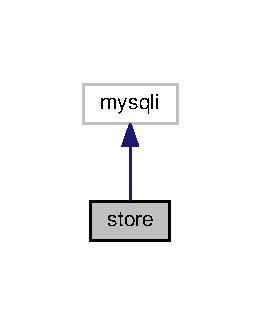
\includegraphics[width=125pt]{classstore__inherit__graph}
\end{center}
\end{figure}


Collaboration diagram for store\+:
\nopagebreak
\begin{figure}[H]
\begin{center}
\leavevmode
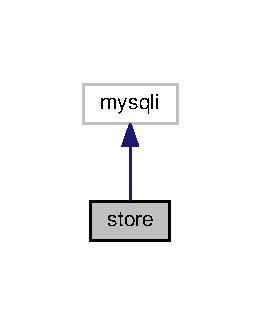
\includegraphics[width=125pt]{classstore__coll__graph}
\end{center}
\end{figure}
\subsection*{Public Member Functions}
\begin{DoxyCompactItemize}
\item 
\hypertarget{classstore_ac6766462e1ba4cf747c89153c158e856}{}{\bfseries \+\_\+\+\_\+construct} (\$u, \$p, \$h= \textquotesingle{}localhost\textquotesingle{}, \$d=false)\label{classstore_ac6766462e1ba4cf747c89153c158e856}

\item 
\hypertarget{classstore_a65f535dfea7bcca33de5078d2bd8f18a}{}{\bfseries query} (\$sql)\label{classstore_a65f535dfea7bcca33de5078d2bd8f18a}

\item 
\hypertarget{classstore_a5ba951e504b410d9442d120e9492393c}{}{\bfseries real\+\_\+escape\+\_\+string} (\$s)\label{classstore_a5ba951e504b410d9442d120e9492393c}

\item 
\hypertarget{classstore_ac69e064cf1e0228d17a98c91d19bc627}{}{\bfseries describe} (\$t)\label{classstore_ac69e064cf1e0228d17a98c91d19bc627}

\item 
\hypertarget{classstore_ac6766462e1ba4cf747c89153c158e856}{}{\bfseries \+\_\+\+\_\+construct} (\$u, \$p, \$h= \textquotesingle{}localhost\textquotesingle{}, \$d=false)\label{classstore_ac6766462e1ba4cf747c89153c158e856}

\item 
\hypertarget{classstore_ac69e064cf1e0228d17a98c91d19bc627}{}{\bfseries describe} (\$t)\label{classstore_ac69e064cf1e0228d17a98c91d19bc627}

\item 
\hypertarget{classstore_a0204fa2a45127ada1589be8e22592522}{}{\bfseries create\+Table} (\$e)\label{classstore_a0204fa2a45127ada1589be8e22592522}

\item 
\hypertarget{classstore_a46e1b2faa9560a512788cc1bf437e047}{}{\bfseries change\+Table} (\$e)\label{classstore_a46e1b2faa9560a512788cc1bf437e047}

\item 
\hypertarget{classstore_a7e1de9852edc997e475aac1f1597730e}{}{\bfseries \+\_\+\+\_\+construct} (\$u, \$p, \$d=false, \$h= \textquotesingle{}localhost\textquotesingle{})\label{classstore_a7e1de9852edc997e475aac1f1597730e}

\item 
\hypertarget{classstore_ac69e064cf1e0228d17a98c91d19bc627}{}{\bfseries describe} (\$t)\label{classstore_ac69e064cf1e0228d17a98c91d19bc627}

\item 
\hypertarget{classstore_a65f535dfea7bcca33de5078d2bd8f18a}{}{\bfseries query} (\$sql)\label{classstore_a65f535dfea7bcca33de5078d2bd8f18a}

\item 
\hypertarget{classstore_a5ba951e504b410d9442d120e9492393c}{}{\bfseries real\+\_\+escape\+\_\+string} (\$s)\label{classstore_a5ba951e504b410d9442d120e9492393c}

\end{DoxyCompactItemize}
\subsection*{Public Attributes}
\begin{DoxyCompactItemize}
\item 
\hypertarget{classstore_a72e10895f184f64e4fccb37473f8d749}{}{\bfseries \$error}\label{classstore_a72e10895f184f64e4fccb37473f8d749}

\end{DoxyCompactItemize}


The documentation for this class was generated from the following files\+:\begin{DoxyCompactItemize}
\item 
lib/mysql.\+php\item 
lib/pgsql.\+php\item 
lib/mysqli.\+php\end{DoxyCompactItemize}

\chapter{File Documentation}
\hypertarget{dbo_8php}{}\section{lib/dbo.php File Reference}
\label{dbo_8php}\index{lib/dbo.\+php@{lib/dbo.\+php}}


D\+B\+O Class definitions.  


\subsection*{Classes}
\begin{DoxyCompactItemize}
\item 
class \hyperlink{classentity}{entity}
\begin{DoxyCompactList}\small\item\em object used to represent either a connection to a database table or the result of a join \end{DoxyCompactList}\item 
class \hyperlink{classconstraint}{constraint}
\begin{DoxyCompactList}\small\item\em object used to define a simple constraint \end{DoxyCompactList}\item 
class \hyperlink{classfilter}{filter}
\begin{DoxyCompactList}\small\item\em object containing a set of constraints \end{DoxyCompactList}\end{DoxyCompactItemize}


\subsection{Detailed Description}
D\+B\+O Class definitions. 


%--- End generated contents ---

% Index
\backmatter
\newpage
\phantomsection
\clearemptydoublepage
\addcontentsline{toc}{chapter}{Index}
\printindex

\end{document}
